\chapter{Przeprowadzone badania}
W niniejszym rozdziale przedstawiono oraz omówiono badania przeprowadzone w celu ewaluacji wydajności interfejsów API implementowanych z wykorzystaniem porównywanych technologii. Każde z wykonanych badań oparte jest o scenariusz testowy określony w ramach sekcji \ref{sec:scenariusze-badawcze}, a także dotyczy odmiennych aspektów działania usługi sieciowej interfejsu programowania aplikacji. W kojenych sekcjach tego rozdziału w sposób szczegółowy opisano podjęte czynności badawcze, zwizualizowano rezultaty każdej z ewaluacji, dokonano analizy statystycznej, a także sformułowano wnioski.

\section{Wpływ zastosowanego systemu bazodanowego na efektywność działania interfejsu API}
W ramach badania zobserwowano zmianę wydajności działania interfejsów programowania aplikacji względem skomunikowanego z nim systemu bazodanowego. Wykorzystano cztery najpopularniejsze relacyjne systemy baz danych (tj. MySQL, SQL Sever, PostgreSQL oraz SQlite), a także jeden system nierelacyjny (tj. MongoDB). Interfejsy programowania aplikacji komunikujące się z poszczególnymi systemami bazodanowymi poddawane były coraz to większemu obciążeniu, poprzez zwiększanie liczby procesów generujących żądania.

Pierwszą czynnością wykonaną w ramach ewaluacji było spełnienie warunków początkowych dotyczących podjęcia czynności badawczych. Warunki te, uwzględniały realizację testów funkcjonalnych, gwarantujących poprawność działania punktów końcowych interfejsu programowania aplikacji. Ponadto, przeprowadzenie tego rodzaju testów pozwoliło na określenie progów tolerancji oraz frustracji wykorzystywanych w kontekście wyliczania wskaźnika wydajności aplikacji APDEX. Ewaluacja funkcjonalna, polegała na uruchomieniu testu uwzględniającego 30 współbieżnie pracujących wątków oprogramowania JMeter, które wysyłały żądania w kierunku punktów końcowych API w czasie 10 minut.

Poczynione zostały dwa następujące założenia:
\begin{itemize}
    \item generowanie żądań przez 30 współbieżnych procesów jest interpretowane jako funkcjonowanie interfejsu programowania aplikacji w standardowych warunkach pracy
    \item ogólna ocena wydajności systemu, a także progi uwzględniane w ramach wskaźnika APDEX generowane są na podstawie tylko tych punktów końcowych, które poddawane są ewaluacji
\end{itemize}

Na wykresie \ref{fig:wykres-testy-funkcjonalne-dotnet} przedstawiono zagregowane względem punktów końcowych, czasy odpowiedzi na żądanie w przypadku interfejsu programowania aplikacji zaimplementowanego z wykorzystaniem środowiska C\#/.NET, a także komunikującego się z bazą danych SQL Server.

\begin{figure}[ht]
    \centering
     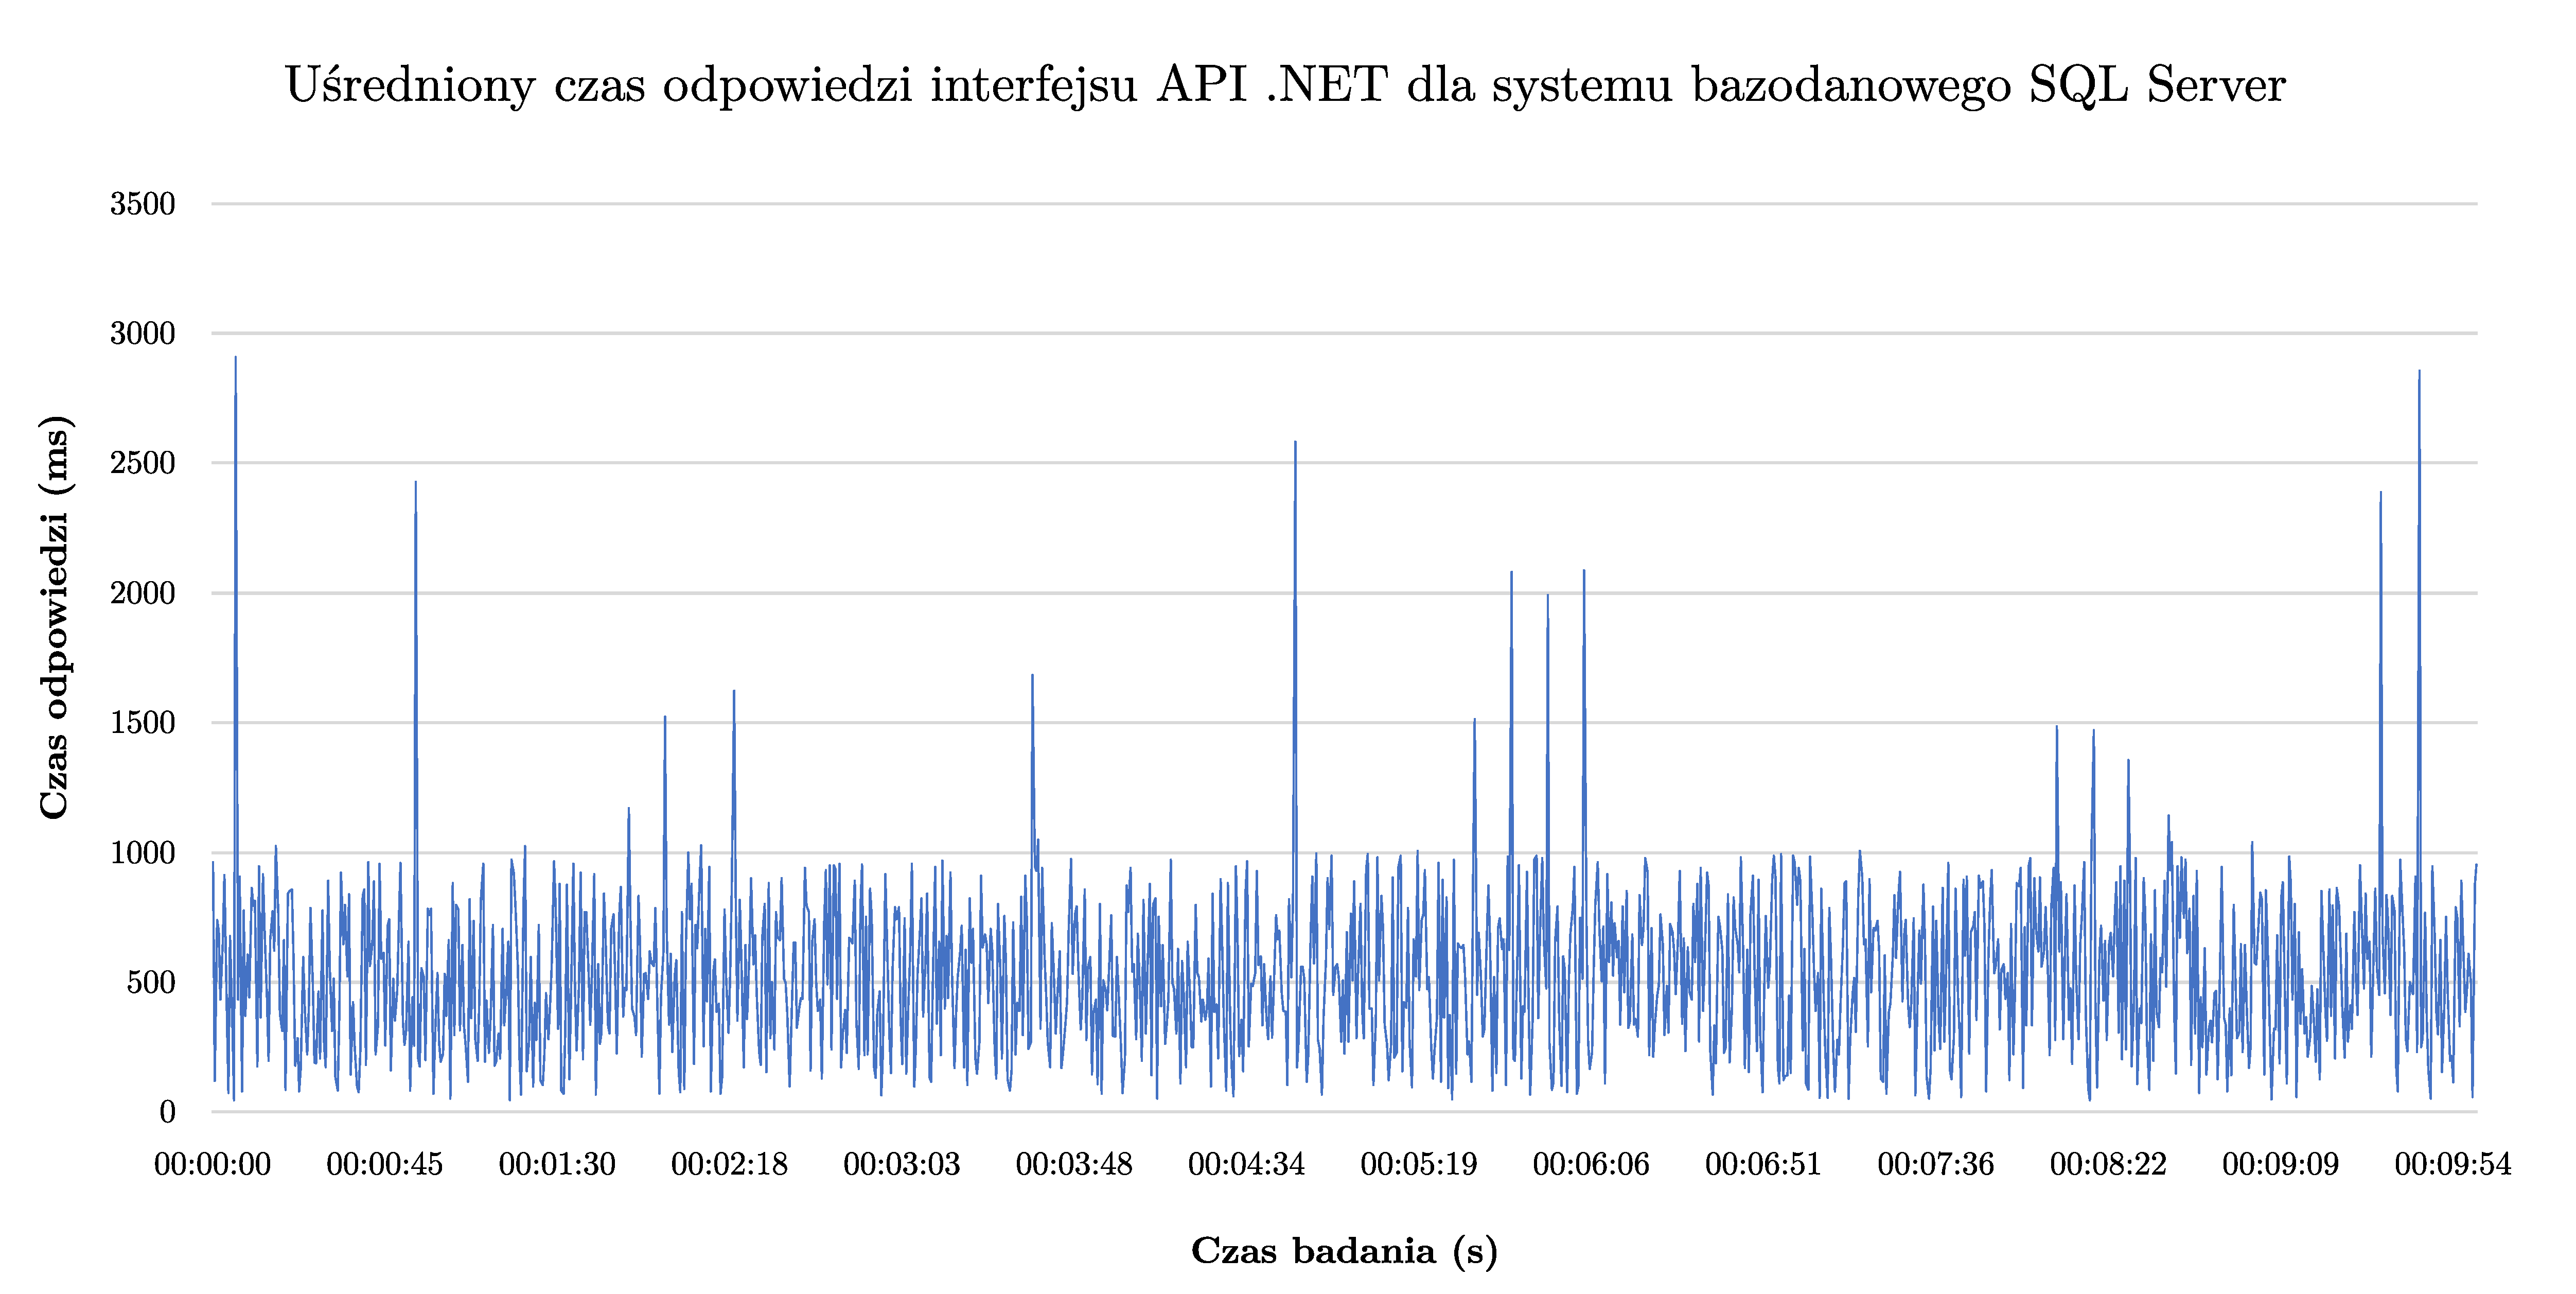
\includegraphics[width=\linewidth]{rys05/testy-funkcjonalne-dotnet.pdf}
    \caption{Czas odpowiedzi na żądanie dla konfiguracji .NET/SQL Server w kontekście testu funkcjonalnego}
    \label{fig:wykres-testy-funkcjonalne-dotnet}
\end{figure}

Na podstawie uzyskanych danych, zdefiniowano progi tolerancji oraz frustracji, wykorzystywane jako punkty odniesienia przy kalkulacji wartości wskaźnika APDEX. Wartości te, ustalono poprzez rosnące posortowanie zbioru czasów odpowiedzi API, a następnie symetryczny podział dwupunktowy. Operacja wykonana została dla każdego z porównywanych systemów bazodanowych w obrębie obu technologii implementacyjnych dotyczących interfejsów API.

Uzyskane przedziały satysfakcji, tolerancji oraz frustracji względem każdego systemu bazodanowego oraz technologii tworzenia API zostały zobrazowane na wykresach \ref{fig:apdex-dotnet} oraz \ref{fig:apdex-nodejs}.

\begin{figure}[ht]
    \centering
     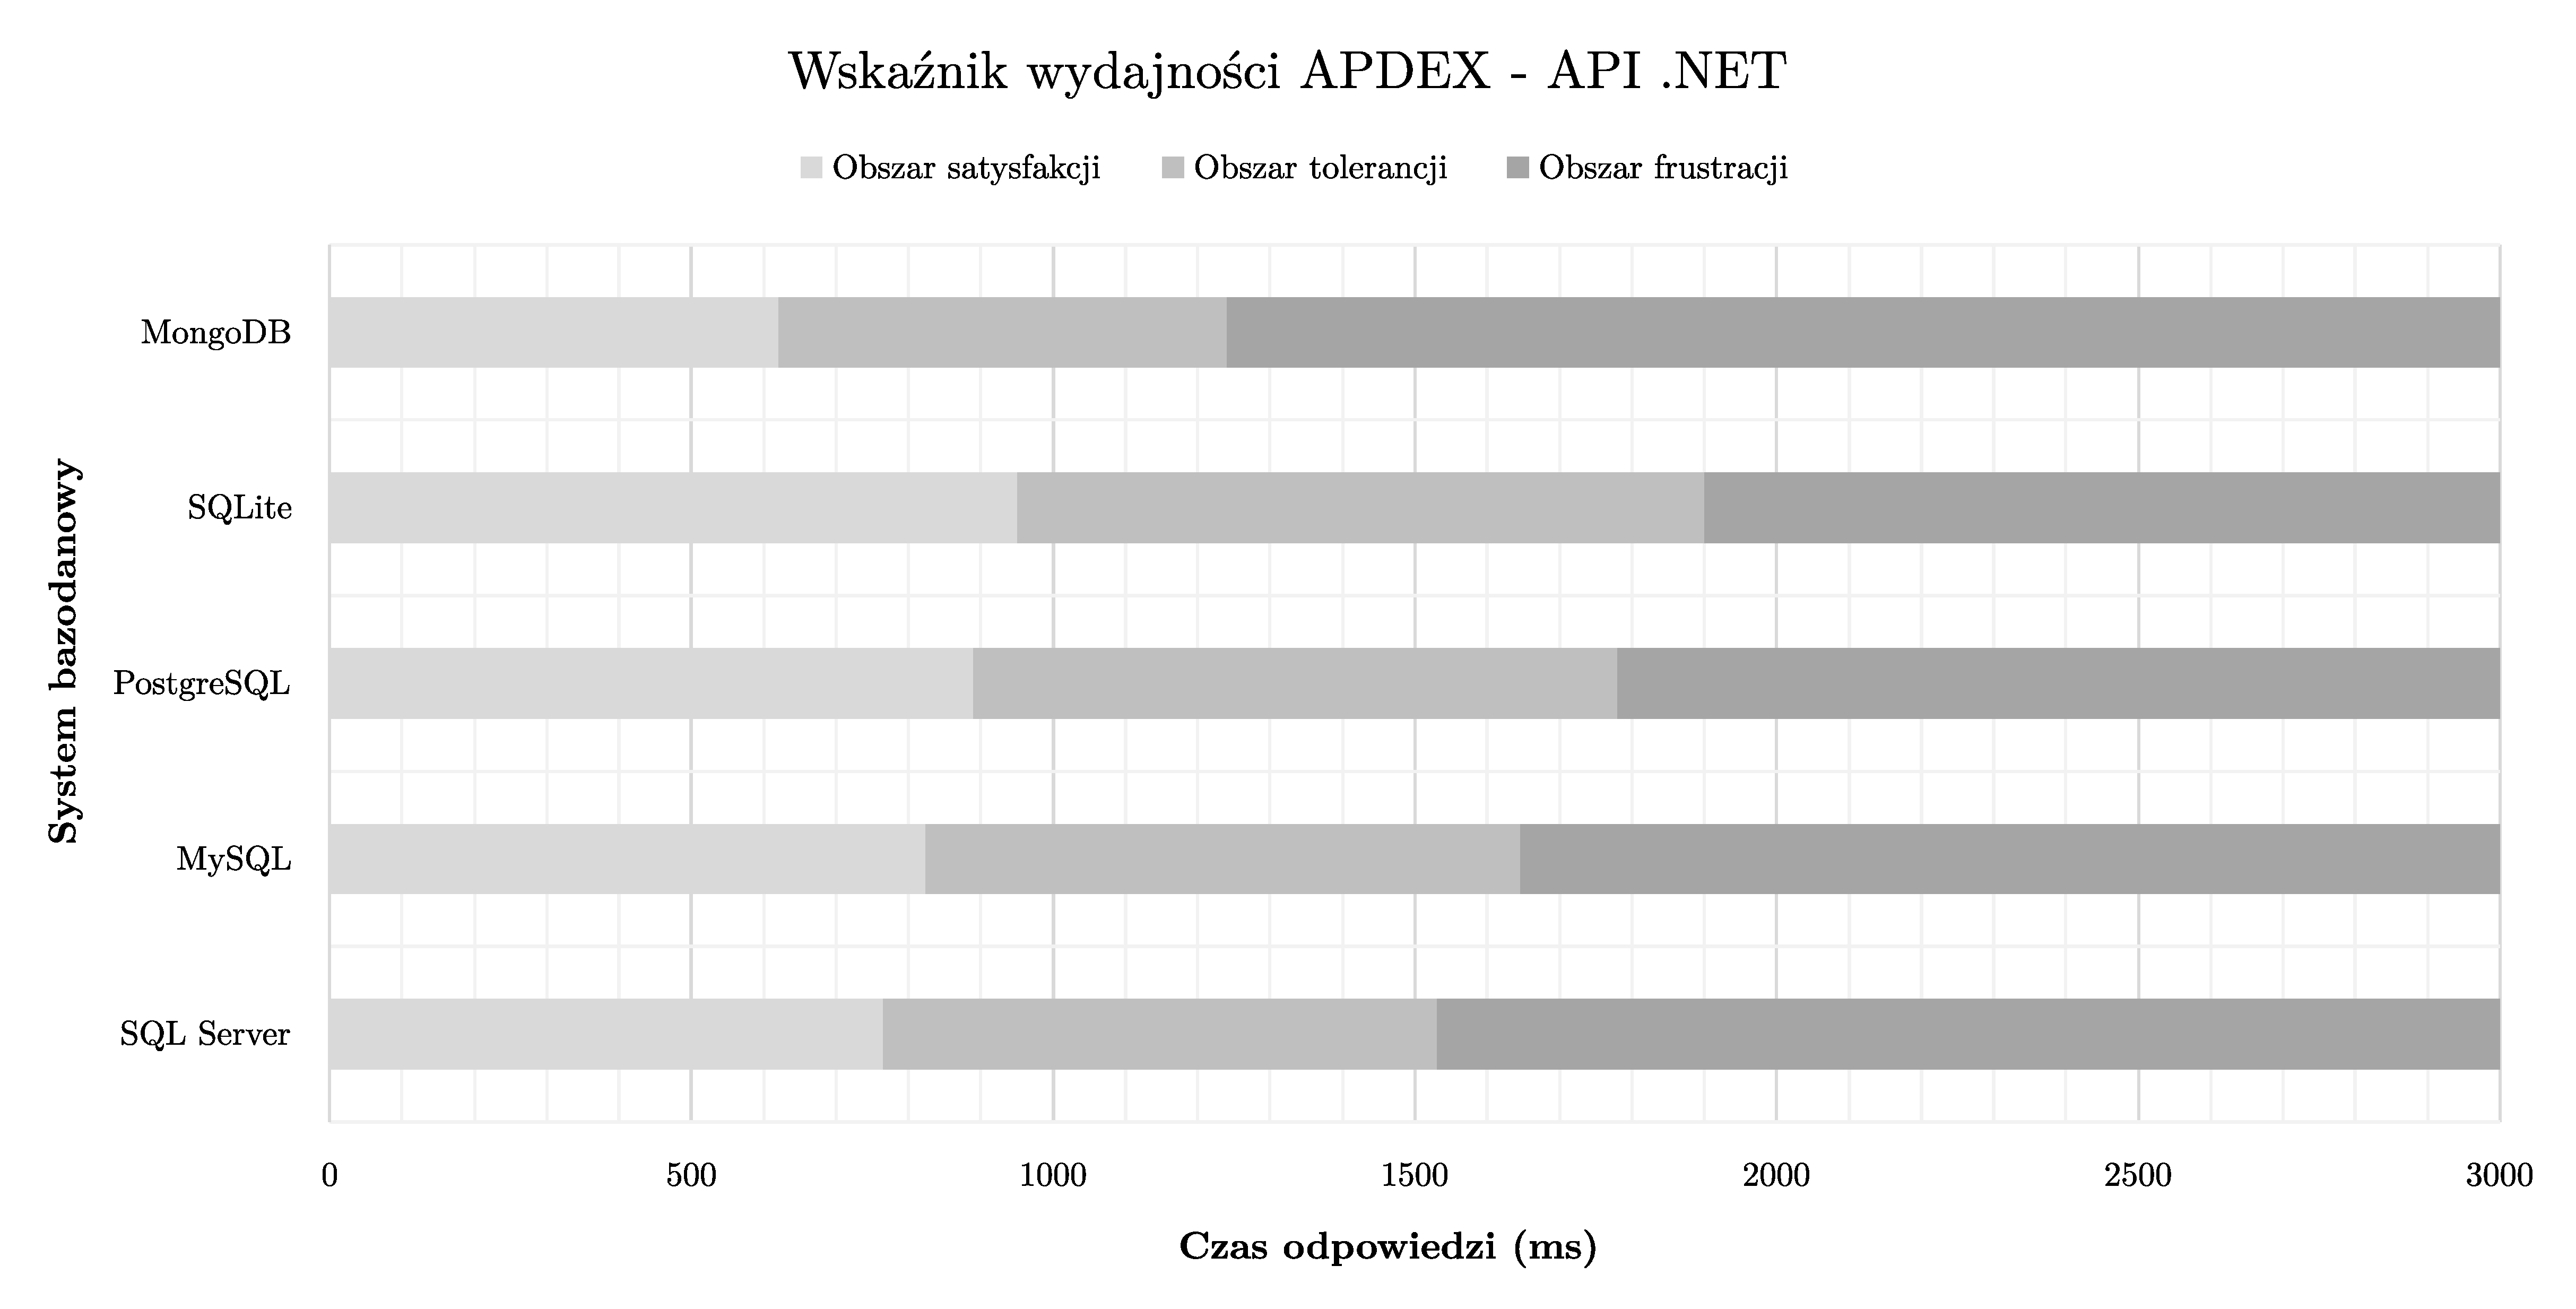
\includegraphics[width=\linewidth]{rys05/apdex-dotnet.pdf}
    \caption{Obszary satysfakcji, tolerancji oraz frustracji wskaźnika APDEX względem poszczególnych systemów bazodanowych dla API zaimplementowanego w C\#}
    \label{fig:apdex-dotnet}
\end{figure}

\begin{figure}[ht]
    \centering
     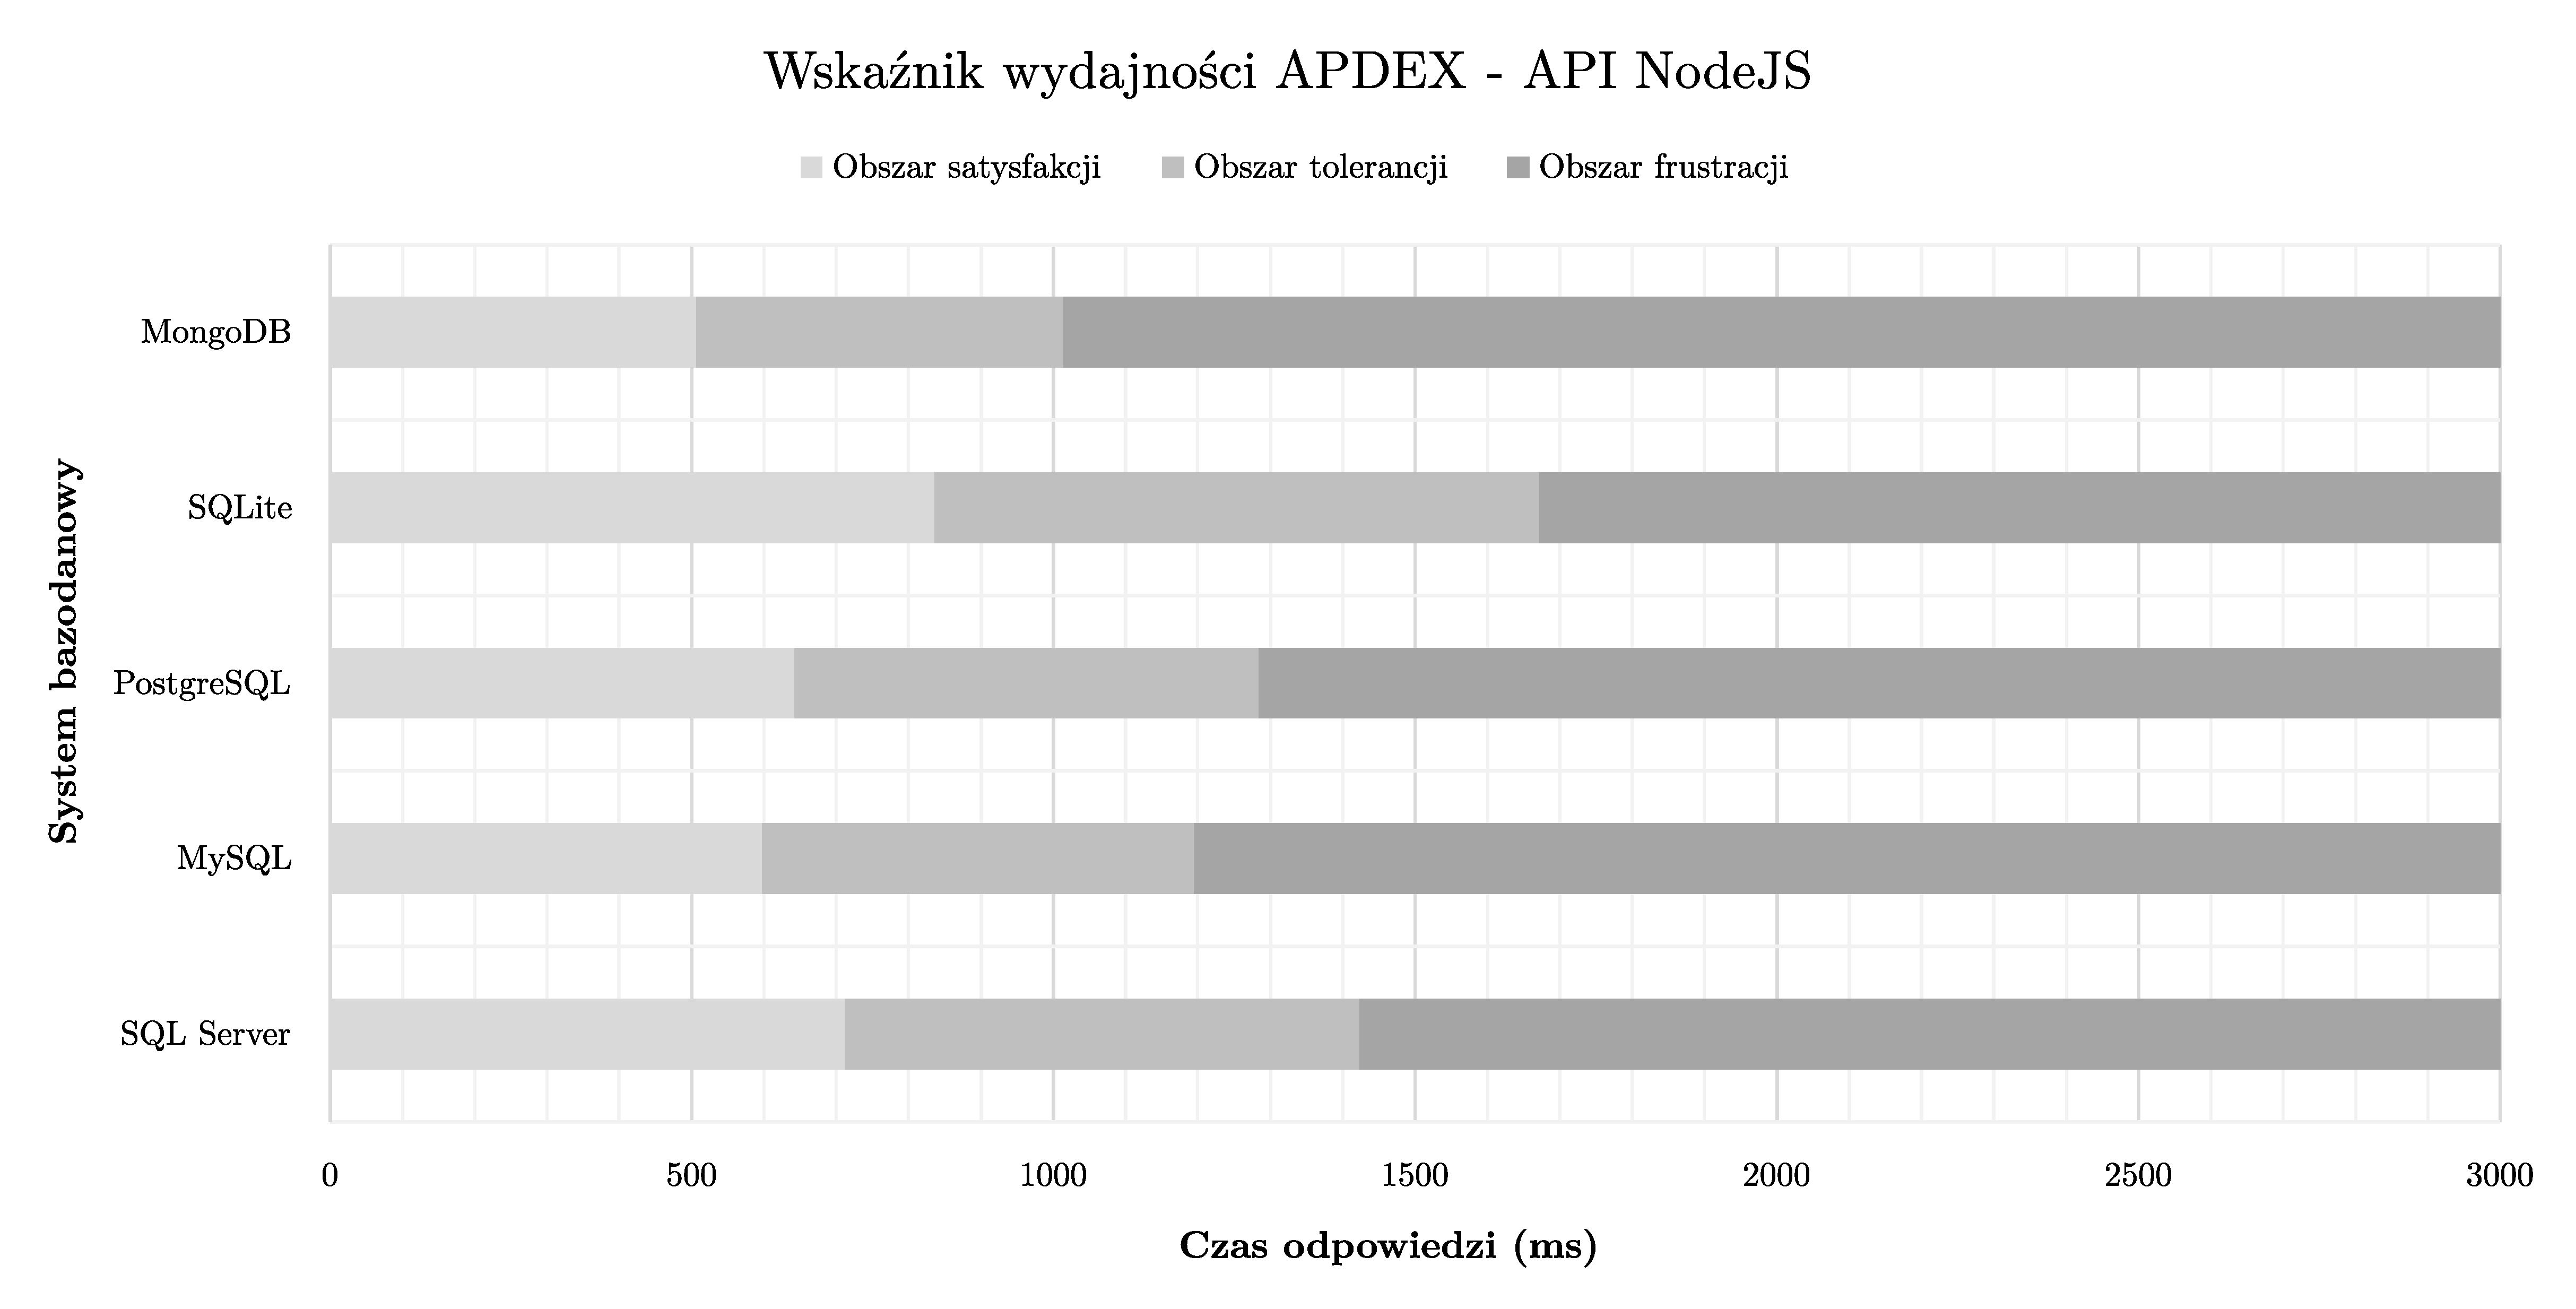
\includegraphics[width=\linewidth]{rys05/apdex-nodejs.pdf}
    \caption{Obszary satysfakcji, tolerancji oraz frustracji wskaźnika APDEX względem poszczególnych systemów bazodanowych dla API zaimplementowanego w JavaScript}
    \label{fig:apdex-nodejs}
\end{figure}

\section{Wpływ zastosowanej technologii programistycznej na wydajność realizacji operacji współbieżnych}
\section{Wpływ zastosowanej technologii programistycznej na efektywność obsługi operacji asynchronicznych}
\section{Wpływ implementacji wzorca projektowego podziału odpowiedzialności na wydajność obsługi żądania klienta}
\section{Porównanie efektywności obsługi żądań klienckich w stałym czasie z uwzględnieniem odmienneych implementacji mechanizmów pamięci podręcznej}
\section{Zmienność wydajności interfejsu API wdrożonego na generycznej oraz dedykowanej platformie chmurowej}